\section{Courbes de \cite{hoppe_impedance_1995}}
\label{sec:annexe:hoppe}
Cette section référence les résultats de \cite{hoppe_impedance_1995}. 


Dans ce livre, la condition d'impédance est de la forme \(\hat{\vE}_t = \hat{\mathfrak{Z}} \hat{\vH}_t\) alors que dans cette thèse, la condition d'impédance est de la forme \(\hat{\vE}_t = \hat{\mZ} \eta_0\left(\vn \pvect \hat{\vH}_t\right)\), \gls{phy-eta_zero} étant l'impédance du vide.

La relation entre les deux matrices est
\begin{equation}
  \hat{\mathfrak{Z}} = \eta_0\hat{\mZ}\begin{bmatrix}0&1\\-1&0\end{bmatrix}
\end{equation}

La figure \ref{fig:annex:hoppe:p33} représente la partie imaginaire du symbole de l'opérateur d'impédance pour un plan infini. La courbe \textit{Exact} correspond au symbole, \textit{SIBC} à Leontovich, \textit{Polynomial} à la CIOE CI4 et \textit{Ratio} à la CIOE CI3.

\begin{figure}[h!tb]
    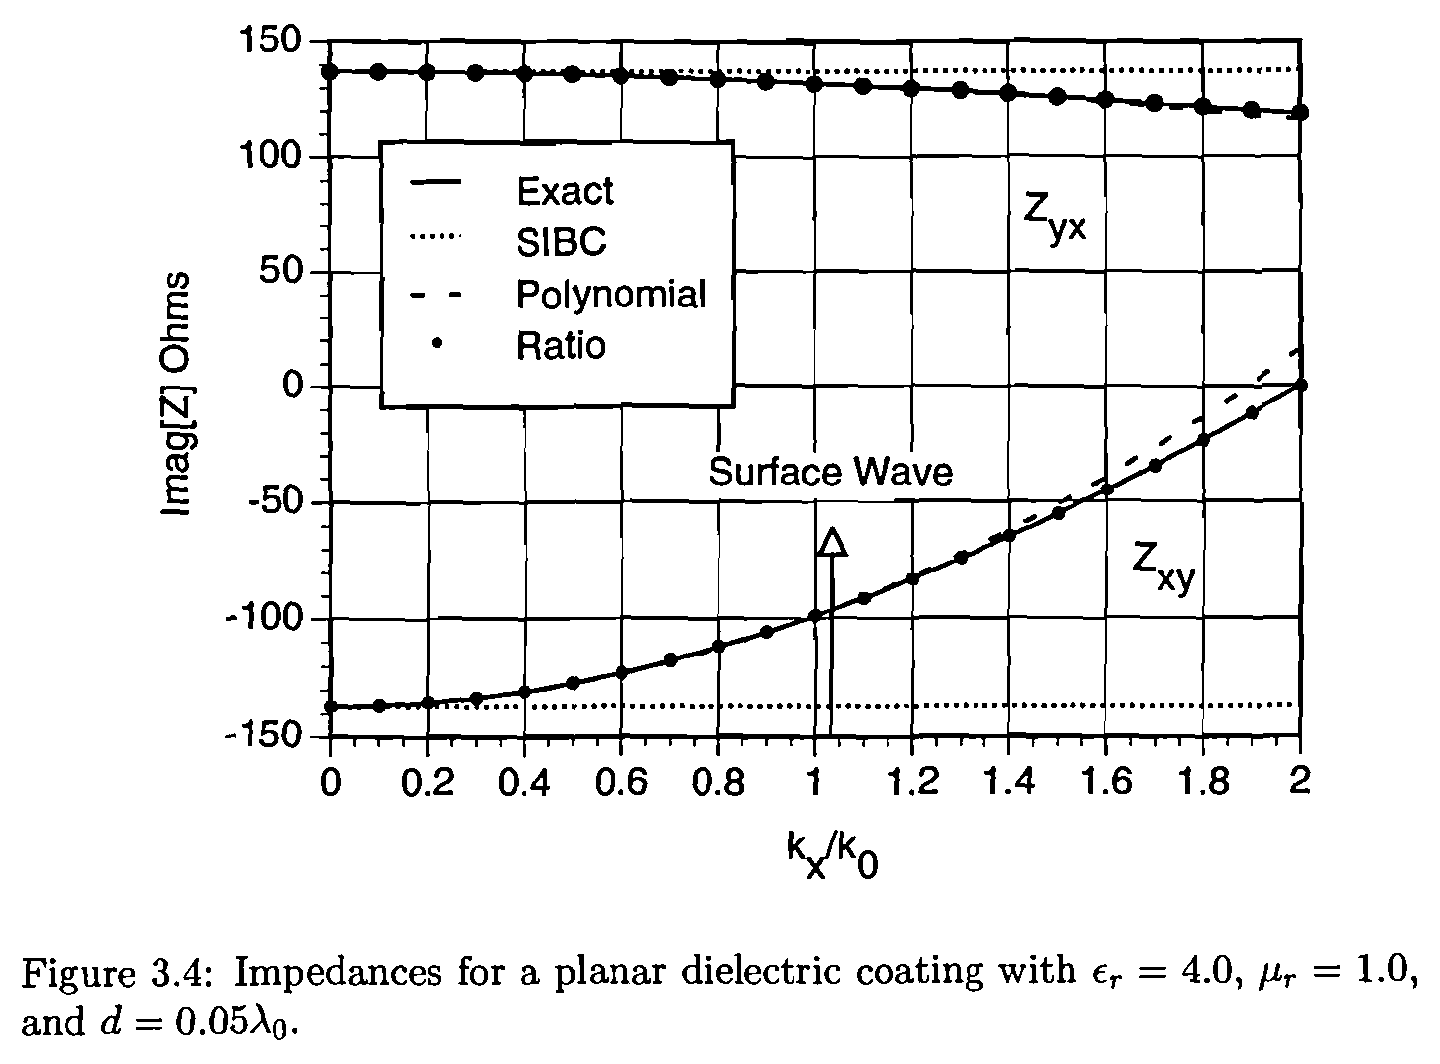
\includegraphics[width=0.99\textwidth]{images/hoppe/p33_imp_cylindre.png}
    \caption{Courbes de la page 33 de Hoppe Rahmat-Samii 1995}
    \label{fig:annex:hoppe:p33}
\end{figure}

La figure \ref{fig:annex:hoppe:p62} représente la partie imaginaire du symbole de l'opérateur d'impédance  pour un cylindre. La courbe \textit{Exact} correspond au symbole, \textit{HOIBC Planar} à la CIOE CI3 et \textit{HOIBC Curvature} à la CIOE CI6.

\begin{figure}[h!tb]
    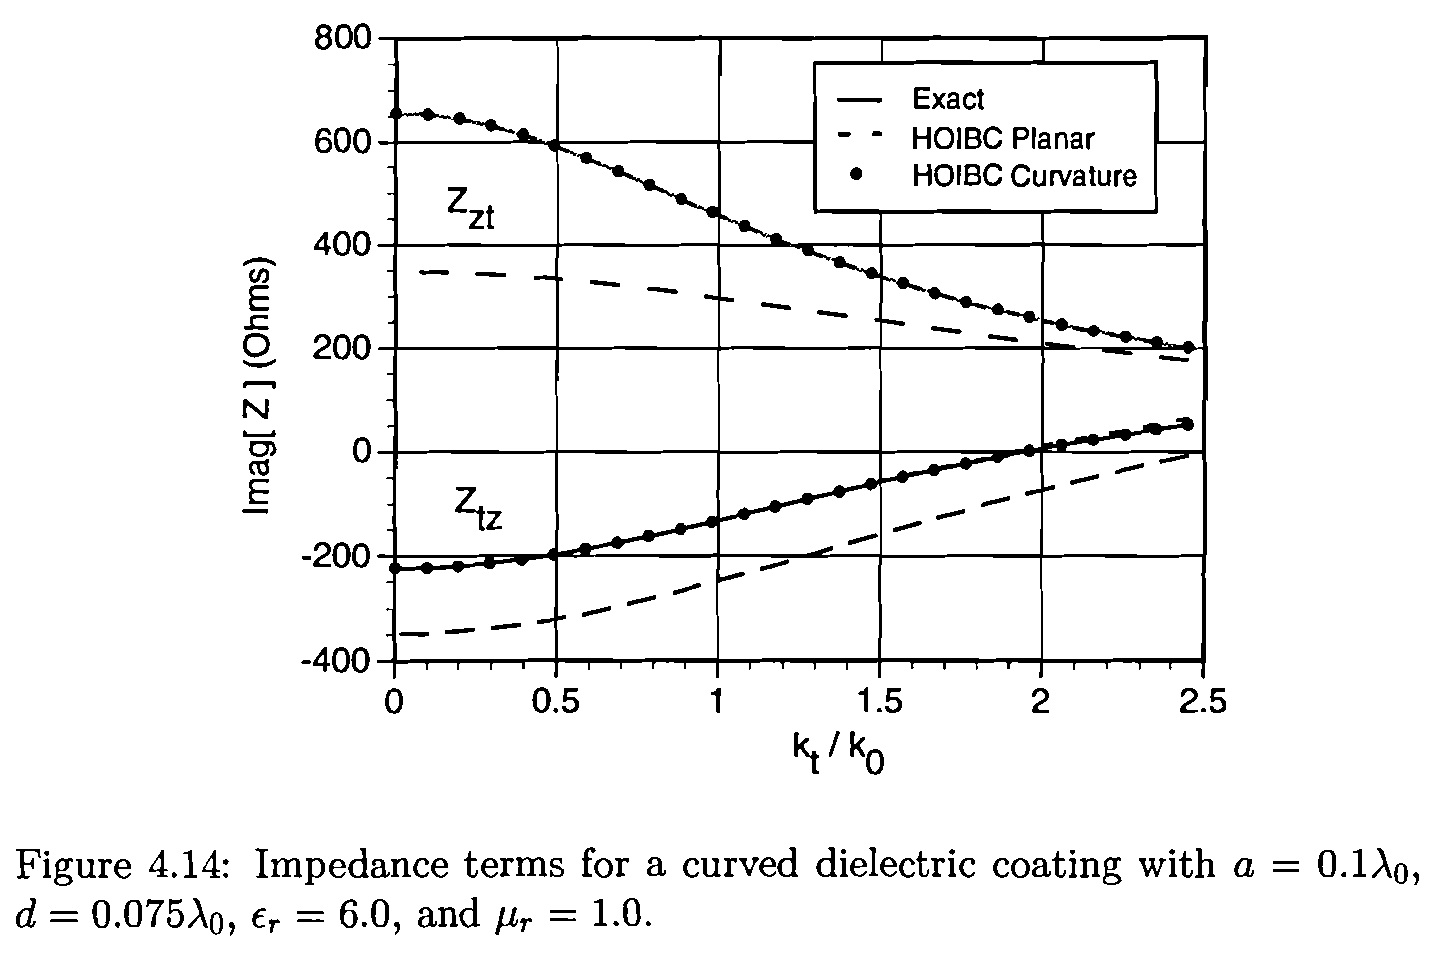
\includegraphics[width=0.99\textwidth]{images/hoppe/p62_imp_cylindre.png}
    \caption{Courbes de la page 62 de Hoppe Rahmat-Samii 1995}
    \label{fig:annex:hoppe:p62}
\end{figure}
